\chapter{Fundamentação Teórica}

\section{Sistemas Computacionais}

Os sistemas computacionais tomaram conta da sociedade atual, o uso de tecnologias computacionais vem tendo muito espaço na comunidade, seja fazendo uso de um computador pessoal, smartphone ou um tablet. Sendo assim, tais dispositivos foram criado essencialmente para satisfazer as necessidades das empresas de forma a garantir e resolver seus problemas organizacionais, ou seja a criação de uma ferramenta que possa armazenar e cruzar dados e informações sem que sejam necessárias pilhas de papéis. Estes sistemas garantem às empresas a possibilidade de atingir mercados em locais mais distantes. \cite{MATTIOLI2020}.

Destaca-se, que o sistema da informação é um tipo especializado de sistema, que pode ser definido de várias formas. Com isso, pode-se entender que sistemas são séries de elementos ou componentes inter-relacionados que coletam entrada de dados, manipulando-os, processando-os, disseminando a saída dos dados e informações, fornecendo assim um mecanismo de \textit{feedback}. \cite{STAIR2008}.

Atualmente a palavra \textbf{sistema} é mal utilizada, usa-se de forma indiscriminada e sem qualquer tipo de fundamento, ou ainda, é usada para expressar determinadas situações dentro de um software, principalmente nos meios empresariais conforme explica \cite{ROSSINI2006}.

Diante disso, é importante conceituar dados, sendo estes como fatos básicos, por exemplo, o nome e a quantidade de horas trabalhadas em uma semana de um funcionário, quantidade de peça em estoque ou pedidos. Importante mencionar que as informações são compostas por um conjunto de fatos organizados de modo a terem valor adicional, além do valor dos fatos propriamente ditos. Portanto, quando dados são organizados ou alcançados de maneira significativa, se transformam em informações. \cite{STAIR2008}.

Conforme informações acima dispostas, apesar do termo sistema estar muito difundido e utilizado muitas vezes de forma leviana, seu significado é bastante preciso. Um sistema é um conjunto de elementos que trabalham de forma integrada a atingir uma ou mais finalidades.
Para que o sistema funcione corretamente, é necessário transformar dados em informações de forma que seus objetivos sejam alcançados, desde a finalidade única de cada elemento até a totalidade das funcionalidades integradas do mesmo.
Com base nisso, na sequência será abordado o assunto referente ao gerenciamento de ordem de manutenção.

\section{Computação Verde}

Computação ou TI Verde é um conjunto de iniciativas de investimento na implantação, uso e gerenciamento a fim de minimizar o impacto negativo ambiental na área de tecnologia da informação. \cite{CQP_MMD_2020}.

O investimento de capital em computação verde é composto por três dimensões: estrutural, humano e relacional.
O capital estrutural refere-se a infraestrutura da TI que engloba \textit{hardware}, \textit{software}, redes e tecnologia da informação. O capital humano é a capacidade e experiência dos profissionais de TI a respeito de conservação de energia em tecnologia e desenvolvimento pessoal com capacidades em TI verde, obtida através de treinamento e estudos. Por último, o capital relacional envolve o gerenciamento da TI verde e a relação das organizações com seus parceiros e usuários, implementando conceitos de proteção ambiental em produtos e serviços. \cite{CQP_MMD_2020}.

Com isso, a adoção das práticas de TI verde propicia uma operação mais sustentável às organizações, gerando economia com energia, papel, água, transporte, espaço físico, manutenção e descarte, proporcionando assim valor tanto para a organização quanto para a sociedade \cite{TallesMoura2017}.

\section{Planejamento e Gerenciamento de Projetos de Software}

Um projeto é um empreendimento temporário que objetiva criar um produto, resultado ou serviço único, que no caso de projeto de software é o sistema em funcionamento \cite{Julia_Mara_2018}.

Os projetos de software apresentam particularidades principalmente por desenvolver produtos incompreensíveis e pela dificuldade do seu gerenciamento, além da falta de comunicação entre os gerentes/desenvolvedores e os clientes/usuários \cite{Prado1999}. As etapas de desenvolvimento seguem um ciclo de vida com fases próprias, tais como a especificação de requisitos, análise, projeto, implementação, testes e implantação \cite{Ralf_Teresa_Erica2018}.

A competitividade e os avanços tecnológicos provocaram um aumento na exigência de qualidade e na complexidade de decisões administrativas. Para obter êxito em um projeto é necessário planejar e gerenciar com eficiência a execução de diversas atividades independentes, pois o grau de risco e incerteza quanto ao sucesso do projeto são elevados \cite{Maria_Isabel_2001}.

Para gerir um projeto, é possível utilizar modelos mais prescritivos como o PMBoK, mais adaptativos como o Scrum ou híbridos.
Os modelos prescritivos possuem uma estrutura formal de elementos do processo como atividades e tarefas, um fluxo de trabalho que descreve como cada um destes elementos deve ocorrer e como eles são relacionados. A busca pela estrutura e a ordem é uma característica importante deste tipo de modelo, que normalmente são compostos por \textit{frameworks} como PMBoK, PRINCE2 e IPMA\cite{Julia_Mara_2018}.
Enquanto os modelos prescritivos presam principalmente pela metodologia e pelo fluxo dos processos, modelos adaptativos como os oriundos do manifesto ágil, são focados na interação entre os usuários no processo de construção do produto através de uma abordagem iterativa e adaptativa\cite{Julia_Mara_2018}.
Os métodos ágeis possuem valores fundamentais, que foram definidos no manifesto ágil, de 2001:
\begin{itemize}
	\item Indivíduos e interação entre eles mais que processos e ferramentas;
	\item Software em funcionamento mais que documentação abrangente;
	\item Software em funcionamento mais que documentação abrangente;
	\item Responder a mudanças mais que seguir um plano.
\end{itemize}

A figura \ref{planejamento_21} mostra o ciclo de gerenciamento de projetos de software. O controle atua tanto no planejamento quanto no desenvolvimento, proporcionando desvios que originam ações corretivas. Entretanto, a avaliação ao final do projeto, reabastece o planejamento com novos projetos e ideias, prosseguindo assim em ciclo indeterminado. Já os padrões são definidos a partir dos controles e das avaliações para controlar e planejar o decorrer do projeto.

\begin{figure}[htb]
	\caption{\label{planejamento_21}Planejamento de Projeto}
	\begin{center}
		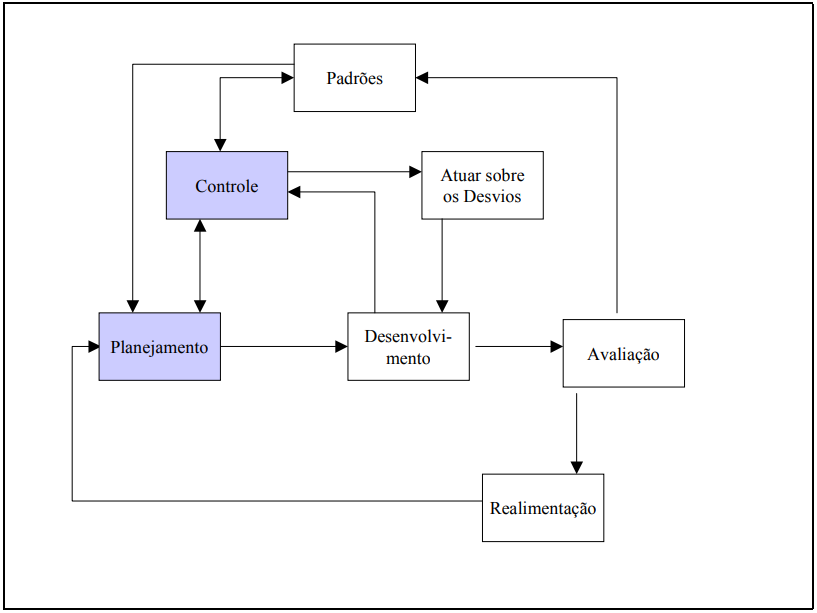
\includegraphics[scale=0.45]{./Figuras/planejamento_projeto.png}
	\end{center}
	\legend{Fonte: \cite{Maria_Isabel_2001}}
\end{figure}

\section{UML}

\section{RUP}

\section{GIT}